\documentclass[twocolumn,a4paper]{article}
\usepackage[a4]{draft}

\usepackage{color}
%%%% Optional package for better font
%\usepackage{txfonts}
\usepackage{cite}
\usepackage{amsmath,amssymb,amsfonts}
\usepackage{algorithmic}
\usepackage{graphicx}
\usepackage{mediabb}
\usepackage{fancybox}

\begin{document}
%date not printed
\date{}

%make title
\title{\Large\bf
Author's GUIDE\\~\\
\large\bf
Preparation of Papers in Two-Column Format}


%for single author
%\author{Center the Authors Names Here \\
%Center the Affiliations Here\\
%Center the City, Stats and Country Here\\
%{\small (it is your option if you want your entire address listed)}}

%for two authors
\author{\normalsize
 \begin{tabular}[t]{c@{\extracolsep{8em}}c}
  \large Author Name& \large Coauthor Name \\
  \\
   Author Department & Coauthor Department \\
   Author Institute  & Coauthor Institute \\
   City, ST~~zipcode & City, ST~~zipcode \\
   author@example.org & coa@example.org
\end{tabular}}

\maketitle

\thispagestyle{empty}

{\small\bf Abstract---
日本語が書ける
Abstract is a brief (50--80 word) synopsis of your paper.
The purpose is to provide a quick outline of your presentation,
giving the reader an overview of the research.
It must be fit within the size allowed, which is about 3\,inches or 7.5\,centimeters.}

\section{Introduction}

These introductions give you basic guidelines for
preparing camera-ready papers for the SASIMI 2025 proceedings.
The instructions assume that you have computer desktop publishing equipment with several fonts.

These instructions have been prepared in the preferred format.
For items not addressed here, please refer to recent issues of IEEE Transactions and simulate,
as closely as possible.



\section{How to Format the Page}

\subsection{Full-Size Camera-Ready Copy}

Prepare Camera-Ready paper in full size format, on A4 size paper.

The length of a short paper is 2 pages, and that of a full paper is 3 to 6 pages, including all figures and tables.


\subsection{Fonts}

The best results will be obtained if your computer word-processor has several font sizes.
Try to follow the font sizes specified in Table I as best as you can.
As an aid to gauging font size, 1\,point is about 0.35\,mm.
Use a proportional, serif font such as Times of Dutch Roman.
Any paper using a font smaller than 9\,pt or larger than 10\,pt for main text will not be included in the proceedings.
See Tab.~\ref{tab:fonts}.

\begin{table}[tb]
\caption{Fonts for Camera-Ready Papers}
\begin{minipage}{8cm}
\def\arraystretch{1.5}\tabcolsep 2pt
\def\thefootnote{a}\footnotesize
\begin{tabular}{l@{~}l@{~~~}l}
\hline
\parbox[c]{7mm}{~\\[-2pt]Font\\Size\\[-7pt]} & Style & Text\\
\hline
 14\,pt&bold     &Paper title\\
 12\,pt&         &Authors' names\\
 10\,pt&         &Authors' affiliations, main text, equations,\\[-5pt]
       &         &first letters in section titles\footnotemark[1]\\
 10\,pt&italic   &Subheadings\\
 ~9\,pt&bold     &Abstract\\
 ~8\,pt&         &Section titles\footnotemark[1], table
                  names\footnotemark[1], first letters in table\\[-5pt]
       &         &captions\footnotemark[1],
                  tables, figure captions, references,\\[-5pt]
       &         &footnotes, text subscripts and superscripts\\
 ~6\,pt&         &Table captions\footnotemark[1], table superscripts\\
\hline
\end{tabular}
\footnotetext[1]{\scriptsize Uppercase}
\end{minipage}
\label{tab:fonts}
\end{table}


\subsection{Formats}

In formatting your A4-size paper, set top margin to 29\,mm (1.14\,inches),
bottom margin to 30\,mm (1.18\,inches), left and right margins to 15\,mm (0.59\,inches).
The column width is 88\,mm (3.46\,inches) with 5\,mm (0.2\,inches) space between the two columns.
You should left- and right-justify your columns.

\section{Figures and Tables}

Place figures and tables at the tops and bottoms of columns.
Avoid placing them in the middle of columns.
Large figures and tables may span across both columns.
Color figures can be included in proceedings,
which should be visible even when the manuscript is printed in monochrome.
Figure captions should be below the figures; table captions should be above the tables.
Avoid placing figures and tables before their first mention in the text.
Use the abbreviation ``Fig.~\ref{fig:fpga}'', even at the beginning of a sentence.

\begin{figure}[t]
  \centering
  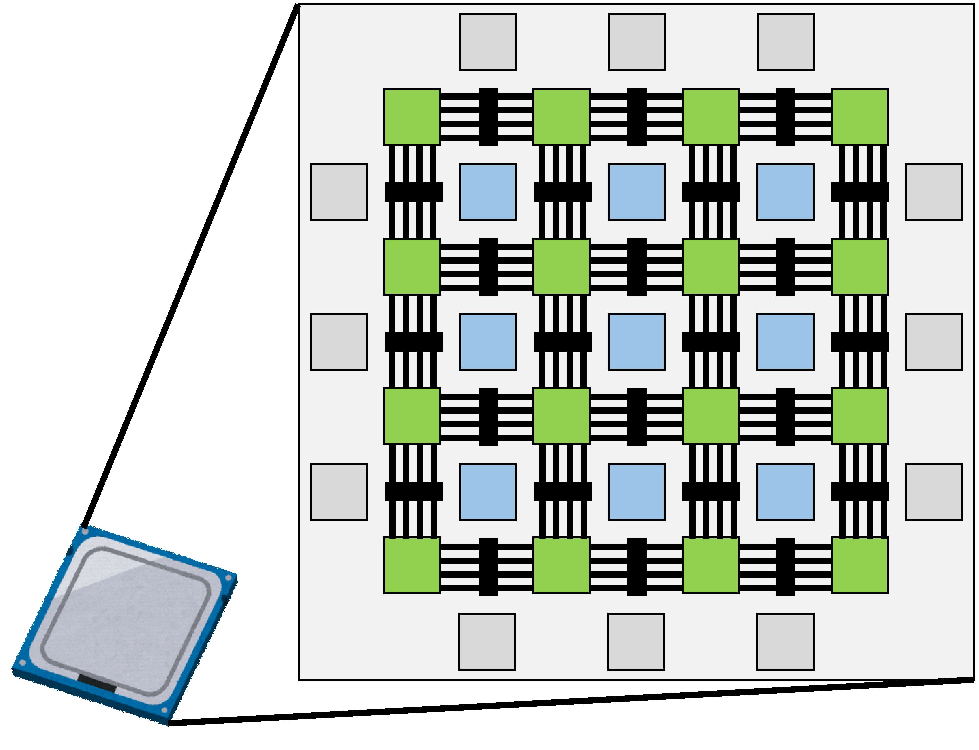
\includegraphics[width=5cm,pagebox=cropbox]{fig/fpga.pdf}
  \caption{図の挿入テスト}
  \label{fig:fpga}
\end{figure}

\section{Helpful Hints}

\subsection{References}
bibtex を使った文献の引用のしかたはこうです\cite{Ullah2022}。


\subsection{Footnotes}
Number the footnotes separately in superscripts. Place the actual
footnote at the bottom of the column in which it is cited. Do not put
footnotes in the reference list.

\section{Summary and Conclusions}
This template will get you through a sample article.

%this is how to do an unnumbered subsection
\section*{\sc Acknowledgements}
This guide is compiled from the author's Guide for the
ASP-DAC'95/CHDL'95/VLSI'95.
This article was written by referring to {\em ``Author's guide --
Preparation of Papers in Two-Column Format for VLSI Symposia on
Technology and Circuits''}, the {\em ``Preparation of Papers in
Two-Column Format for the Proceedings of the 32nd ACM/IEEE Design
Automation Conference''} written by Ann Burgmeyer, IEEE and {\em ``the
template for producing IEEE-format articles using LaTeX''}, written by
Matthew Ward, Worcester Polytechnic Institute.

\footnotesize

\bibliographystyle{myjunsrt}
\bibliography{library}

\end{document}
